\documentclass[journal,10pt,draftclsnofoot,onecolumn]{IEEEtran}
\usepackage[doublespacing]{setspace}
\usepackage[margin=0.75in]{geometry}
\usepackage{graphicx}

\begin{document}

\begin{titlepage}
\newcommand{\HRule}{\rule{\linewidth}{0.4mm}}

\center

\textsc{\Large CS461 Fall 2017 }\\[0.5cm]
\textsc{\large Group 19}\\[0.5cm] % Minor heading such as course title

{\huge\bfseries Software Requirement Specifications for Aerolyzer Python API}\\[0.4cm]

\vfill
\begin{minipage}{0.4\textwidth}
\begin{flushleft}
\large
\textit{Authors}\\
Kin-Ho \textsc{Lam}\\
Logan \textsc{Wingrad}\\
Daniel \textsc{Ross}\\
\end{flushleft}F
\end{minipage}
\vfill
\begin{minipage}{0.4\textwidth}
\begin{flushleft}
\large
\textit{Supervisor}\\
Dr. Kim \textsc{Whitehall}
\end{flushleft}
\end{minipage}

\vfill

\begin{abstract}
Atmospheric aerosols are tiny particles dispersed throughout the atmosphere.
These particles originate from natural sources such as volcanic eruptions, and unnatural sources such as pollution. 
Monitoring atmospheric aerosols is important due to their effects on the atmosphere's chemical composition and radiation distribution.
The presence of aerosols reduces air quality which can potentially lead to health complications such as bronchitis or respiratory inflammation.
One can visibly see the effects of aerosols in the 'Rayleigh scattering effect' which visibly reddens sunsets and sunrises.
Analyzing atmospheric content in the air provides insight on air quality. 
However, existing methods to gather aerosol data such as satellites, planes, and ground-based instruments provide data that are too complex to be useful for the average person to understand or do not provide data fast enough.
Aerolyzer is a web application that uses weather information and acceptable images of the horizon to infer local atmospheric phenomena in the United States. 
The following document details the software requirement specifications for Aerolyzer Aerosol Detection API. The Aerosol Detection API will consist of  python classifiers that shall analyze user submitted images, and remove unacceptable images.
\end{abstract}

\vfill
\vfill
\vfill
{\large10/25/17}
\vfill
\end{titlepage}

\tableofcontents
\clearpage

\begin{singlespace}

\section{Introduction}

\subsection{Purpose}
The Aerolyzer Project aims to deliver a new source of air quality and weather information through leveraging machine learning algorithms to characterize aerosol content in the atmosphere.
When complete, this open-source project shall feature a Python library that uses image classification and third-party weather APIs, displayed with an intuitive web-based user interface.
The Aerolyzer project requires a Python library that identifies images relevant to aerosols, analyzes acceptable images for aerosol content, stores relevant information for trend analysis, and compiles weather information with its aerosol data. 

\subsection{Scope}
Bringing aerosol analysis to a mainstream audience calls for an open-source back-end Python API to perform image analysis.
This front-end UI shall present the Aerolyzer library's weather and air quality inference based on analyzed images or by a requested location.
The UI shall collect user-submitted cell phone images of the horizon, sunset, and sunrise to be fed to the library for analysis.
The Aerolyzer project shall exclusively serve users in the United States.

\subsection{Definitions}
Aerosol: Small particles suspended in the atmosphere.
One can visibly see the effects of aerosols in the 'Rayleigh scattering effect' which visibly reddens sunsets and sunrises. \\

Acceptable image: An acceptable image is defined as an unedited image of the horizon, sunset, or sunrise.
Images used in data collection must have valid EXIF metadata, while the images used in training classifiers only require relevant image content.\\

Horizon: The horizon is defined as the line at which the sky and earth's surface appear to meet.\\

Sunrise: A sunrise is defined as the colors and light visible in the sky produced by the sun's first appearance in the morning.\\

Sunset: A sunset is defined as the colors and light visible in the sky produced when the sun disappears in the evening.\\

EXIF: Exchangeable image file format \\

\section{Project Overview}

\subsection{Product Perspective}
Aerolyzer is an air quality analysis library that will be utilized by users via a mobile web application.
The library takes images of the horizon at dusk or dawn, or a user's ZIP code as input.
Multiple image classifiers will be developed using machine learning with acceptable images selected for training from public sources.
User submitted images will be utilized in the machine learning process if they're deemed acceptable. 

\subsection{Product Functions}
Aerolyzer's web interface will take a user's location, either from a submitted image's EXIF data or a provided ZIP code, as the primary input.
If the user submitted an acceptable image, the results of color analysis on that image are add to the application's data for their ZIP code.
The library then calls on weather API for meteorological data for their ZIP code.
The application then displays all data relevant to the user's ZIP code on their screen in an understandable format.

\section{Users \& Functionality}
\subsection{User Stories}
Users shall either know their current ZIP code or have a mobile device that stores their location in the EXIF data of an image when it's taken.


\subsection{Expected user characteristics}
\begin{enumerate}
\item The user will own a smartphone
\item The user has a general idea of what aerosols are
\item The users shall understand how to use their mobile device to capture an image of the horizon.
\item The users shall have a basic understanding of how to navigate a web browser in order to use the web application.
\item The users shall know the fundamentals of weather conditions, like temperature, wind speed, and humidity.
\end{enumerate}

\subsection{Input Constraints}
\begin{enumerate}
\item The image must be taken on a device with location tracking enabled
\item The image must be unedited and have no filters applied
\item The image must also have exif data
\item The image must contain a horizon
\item The image must contain either a sunset or sunrise
\item The image must be from in the USA
\end{enumerate}

\subsection{Assumptions and Dependencies}
We assume users submitting photos have given permission for having their image stored and used in further processing.
We assume the user is connected to the internet.
We assume that the user's web browser supports the application's interface.
\begin{figure}
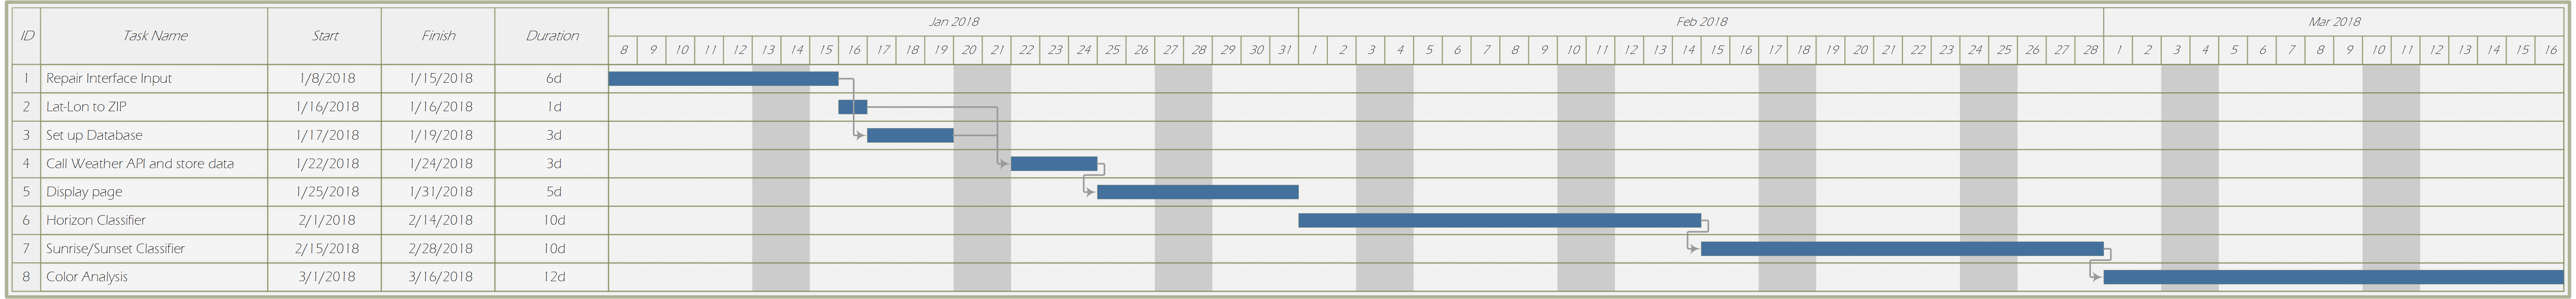
\includegraphics[width=\linewidth]{gantt.png}
\end{figure}
\subsection{External Interfaces}
The library will make external calls to the Weather Underground API for current weather conditions at a certain ZIP code.
The library will also facilitate the storage of images into a external database.
The last external connection is to image classifiers, that will have access to the same database, which will do their classification externally.

\section{Functions}
\subsection{Functions}
\begin{enumerate}
\item Web Application Interface
Trigger: User navigates to the Application site using a Web Browser
Precondition: User has access to a web browser and the internet.
Basic Path:
User opens web browser
User navigates to the Aerolyzer URL in the web browser
System serves start page to the user
Alternative Paths: Users can navigate to the Aerolyzer start page via link
Postcondition: User has access to the application
Exception Paths: If the user isn't connected to the internet or their web browser can't access the page, the use case is abandoned.
\\
\item ZIP code submission
Trigger: User clicks submit on form for ZIP code
Precondition: User's web browser correctly displays the form for ZIP input.
Basic Path:
User types ZIP code in form
User clicks “Submit” button on form
Alternative Paths: See Function 3.) Upload Photo
Postcondition: User is navigated to output page.
Exception Paths: If the submitted ZIP code isn't a valid 5 digit ZIP, the user is notified and the use case is abandoned.
\\
\item Upload Photo
Trigger: User clicks the “Upload a Photo” button
Precondition: Users have a picture from a mobile device and their web browser has access to this photo.
Basic Path:
Alternative Paths:
Postcondition:
Exception Paths: 
\\
\item Extract EXIF
Trigger:
Precondition: Photo has been successfully uploaded as per use case 3
Basic Path: 
Aerolyzer library receives image as input for extraction script.
Script outputs the image's EXIF data as a JSON file.
The JSON file is stored with the image prior to classification.
Alternative Paths: Images and their associated metadata can be added manually to the database.
Postcondition: The central database has access to the image and its metadata.
Exception Paths: None
\\
\item Classify photo
Trigger: A unclassified photo has been added to the central database.
Precondition: The image and its JSON metadata are accessible to the classifier as per use case 4.
Basic Path:
	The image's latitude and longitude are read from the JSON metadata.
	The latitude and longitude are used to identify the image's ZIP code.
The image is checked with the horizon classifier to confirm the presence of a horizon in the image.
If Horizon is confirmed, the image is checked using a sunset/sunrise classifier to confirm the presence of a sunset or sunrise.
	The image is stored in the database with it's content and ZIP code identifying it.
Alternative Paths: The image is checked with the horizon classifier and the image isn't confirmed to have the horizon in it. The user is notified, the image isn't stored, and the ZIP code is used in use case 6.
Postcondition: The user's image is stored and categorized for further use.
Exception Paths: The latitude and longitude in the image JSON data aren't in the United States, the user is notified and the use case abandoned.
\\
\item Call Weather API
Trigger: The user's ZIP code is received.
Precondition: The user submitted their ZIP code as per use case 2 or The user submitted an image that was successfully identified as per use case 5.
Basic Path:
A request is made to the weather API for data on the recieved ZIP code.
The data received from the weather API is stored in the central database under the ZIP code it pertains to.
Alternative Paths: None
Postcondition: The central database has meteorological and astronomical data for a ZIP code.
Exception Paths: If data is unable to be retrieved from the weather API, an error message will be displayed.
\\
\item Identify Aerosols
Trigger: The user's ZIP code and their submitted image is received.
Precondition: The user submitted an image that was successfully identified as per use case 5.
Basic Path:
The colors in the image are analyzed.
The analysis returns the type of aerosol most likely to cause the colors in the image.
The type of aerosol and the current time are stored in the central database under the user's ZIP code.
Alternative Paths: None
Postcondition: The central database has a type of aerosol at a particular time for a certain ZIP code.
Exception Paths: None
\\
\item Display data
Trigger: Use case 6 is completed.
Precondition: The central database has completed any updates in progress on the user's requested ZIP code.
Basic Path: 
All of the most recent data for the user's ZIP code is fetched from the central database.
Alternative Paths:None
Postcondition:The user is taken to a page to display the fetched data.
Exception Paths: None
\end{enumerate}

\subsection{Functionality}
Aerolizer will be a smartphone application that grants its users information on aerosols in the atmosphere based on collected information from images taken by users as well as the exif data that came along with the image. It will use machine learning to analyze the wavelengths of the light refracting through our atmosphere to determine the size of the aerosols in the air. It will then relay the information to the user in a user-friendly UI. 

\section{Performance}
\subsection{Performance Requirements}
When completed, this library shall identify horizons using Aerolyzer's classifier in a test-selection of images with a minimum accuracy of 66\% certainty. Images of horizons that contain sunsets and sunrises shall be identified using Aerolyzer's classifier library with a minimum of 50\% certainty. This certainty shall be verifiable through a series of regression tests to prove detection accuracy.
The library will be able to handle up to 10 image submissions per minute and 500 images at most in a single day.


\nocite{*}
\bibliographystyle{plain}
\bibliography{ref}


\end{singlespace}
\end{document}
